\documentclass[aspectratio=169]{beamer}
\usepackage[square,numbers]{natbib}
\bibliographystyle{apalike}
\title[Stiby Systems Case Presentation]{UX Architecture for Data Collaboration}
\date[]{\today}
\author[]{Henrik Korsgaard}
\institute{DEPARTMENT OF COMPUTER SCIENCE} % Type in A
\usetheme{henrikkorsgaard}

\usepackage{multicol}

\usetikzlibrary{shapes.geometric, shapes.symbols}
\usepackage{tikzpeople}
\usetikzlibrary{arrows.meta}
\usepackage{fontawesome5}
\usepackage{changepage}
\makeatletter
\newbox\@backgroundblock
\newenvironment{backgroundblock}[2]{%
  \global\setbox\@backgroundblock=\vbox\bgroup%
    \unvbox\@backgroundblock%
    \vbox to0pt\bgroup\vskip#2\hbox to0pt\bgroup\hskip#1\relax%
}{\egroup\egroup\egroup}
\addtobeamertemplate{background}{\box\@backgroundblock}{}
\makeatother

\makeatletter
    \newsavebox\restorebox
\newenvironment{restoretext}%
    {\@parboxrestore% 
     \begin{adjustwidth}{-8mm}{-8mm}%
                \begin{lrbox}{\restorebox}%
                \begin{minipage}{\linewidth}%
    }{\end{minipage}\end{lrbox}
        \usebox\restorebox
        \end{adjustwidth}
     }
\makeatother

\begin{document}

\begin{frame}
\maketitle
\end{frame}

\begin{frame}{Outline and focus}
    \begin{columns}
        \begin{column}{0.5\textwidth}
            \begin{itemize}
                \item UX research process
                \item ``Results'' and assumptions
                \item Information design for shared views
                \item Interaction design for collaborative features
                %%\item If time, responsive filtering %% if you cannot execute this within time, then keep
            \end{itemize}
        \end{column}
        \begin{column}{0.5\textwidth}
            As a newly hired UX architect, your initial task is to create an outline for the UX work in a project aimed at improving the UX of the \textbf{collaboration tooling} in an existing online Excel-like table system.\\
            \vspace{1em}
            {\color{HenrikFontLight}\dots assume that you have the necessary budget for it.}
        \end{column}
    \end{columns}
\end{frame}

\begin{frame}{UX Research}
    \begin{description}
        \small
        \item[Discovery:] How, when and why do users collaborate?
        \item[Define:] What are the main user scenarios, information concepts and features?
        \item[Prototype:] User flows, wireframes, key interfaces and features
        \item[Evaluate:] User testing and evaluation
        \item[Integrate:] Plan integration and delivery
        %\item Think aloud evaluation
    \end{description}
    \begin{restoretext}
    \begin{backgroundblock}{7mm}{50mm}
    \centering
    \resizebox{1\textwidth}{!}{%
    \begin{tikzpicture}

        \node[diamond,fill=HenrikDark!2, minimum width = 4.5cm, minimum height = 4.5cm] (d) at (1.1,1) {};
        \node[diamond,fill=HenrikDark!2, minimum width = 4.5cm, minimum height = 4.5cm] (d) at (5.5,1) {};

        \node[signal to=east, signal from=west,shape=signal, draw, minimum width = 2.15cm, minimum height = 0.5cm, fill=white] at (0.1,1) {\tiny Discover};
        \node[signal to=east, signal from=west, shape=signal, draw, minimum width = 2.3cm, minimum height = 0.5cm, fill=white] at (2.2,1) {\tiny Define};
        \node[signal to=east, signal from=west, shape=signal, draw, minimum width = 2.3cm, minimum height = 0.5cm, fill=white] at (4.37,1) {\tiny Prototype};
        \node[signal to=east, signal from=west, shape=signal, draw, minimum width = 2.3cm, minimum height = 0.5cm, fill=white] at (6.54,1) {\tiny Evaluate};
        \node[signal to=east, signal from=west, shape=signal, draw, minimum width = 2.3cm, minimum height = 0.5cm, fill=white] at (8.7,1) {\tiny Integrate}; 
    \end{tikzpicture}
    }
\end{backgroundblock}
\end{restoretext}
\end{frame}


\begin{frame}{UX Research}
    \begin{columns}[t]
        \begin{column}{0.5\textwidth}
            \small
            \textbf{Discover}
            \begin{itemize}
                \item Internal research and analytics
                \item Contextual interviews with users
                \item Observe collaborative task sessions
                \item State-of-art on collaborative applications (CRDT)
            \end{itemize}
        \end{column}
        \begin{column}{0.5\textwidth}
            \small
            \textbf{Define}
            \begin{itemize}
                \item Workshops!
                \item Collaborative task objectives
                \item Scenarios, personas and user journeys (user stories)
                \item Information concepts and architecture
                \item UX quality criteria and KPIs
            \end{itemize}
        \end{column}
    \end{columns}
    \begin{restoretext}
    \begin{backgroundblock}{7mm}{50mm}
    \centering
    \resizebox{1\textwidth}{!}{%
    \begin{tikzpicture}

        \node[diamond,fill=HenrikDark!2, minimum width = 4.5cm, minimum height = 4.5cm] (d) at (1.1,1) {};
        \node[diamond,fill=HenrikDark!2, minimum width = 4.5cm, minimum height = 4.5cm] (d) at (5.5,1) {};

        \node[signal to=east, signal from=west,shape=signal, draw, minimum width = 2.15cm, minimum height = 0.5cm, fill=HenrikDark, white] at (0.1,1) {\tiny Discover};
        \node[signal to=east, signal from=west, shape=signal, draw, minimum width = 2.3cm, minimum height = 0.5cm, fill=HenrikDark, white] at (2.2,1) {\tiny Define};
        \node[signal to=east, signal from=west, shape=signal, draw, minimum width = 2.3cm, minimum height = 0.5cm, fill=white] at (4.37,1) {\tiny Prototype};
        \node[signal to=east, signal from=west, shape=signal, draw, minimum width = 2.3cm, minimum height = 0.5cm, fill=white] at (6.54,1) {\tiny Evaluate};
        \node[signal to=east, signal from=west, shape=signal, draw, minimum width = 2.3cm, minimum height = 0.5cm, fill=white] at (8.7,1) {\tiny Integrate}; 
    \end{tikzpicture}
    }
\end{backgroundblock}
\end{restoretext}
\end{frame}

\begin{frame}{UX Research}
    \begin{columns}[t]
        \begin{column}{0.5\textwidth}
            \small
            \textbf{Prototype}
            \begin{itemize}
                \item User and collaborative flow
                \item Information architecture and layout
                \item Data and view operations 
                \item Real-time collaboration
            \end{itemize}
        \end{column}
        \begin{column}{0.5\textwidth}
            \small
            \textbf{Evaluate}
            \begin{itemize}
                \item Internal review and testing
                \item (informal) user feedback
                \item Think aloud evaluation 
                \item Review UX quality criteria and KPIs
            \end{itemize}
        \end{column}
    \end{columns}
    \begin{restoretext}
    \begin{backgroundblock}{7mm}{50mm}
    \centering
    \resizebox{1\textwidth}{!}{%
    \begin{tikzpicture}

        \node[diamond,fill=HenrikDark!2, minimum width = 4.5cm, minimum height = 4.5cm] (d) at (1.1,1) {};
        \node[diamond,fill=HenrikDark!2, minimum width = 4.5cm, minimum height = 4.5cm] (d) at (5.5,1) {};

        \node[signal to=east, signal from=west,shape=signal, draw, minimum width = 2.15cm, minimum height = 0.5cm] at (0.1,1) {\tiny Discover};
        \node[signal to=east, signal from=west, shape=signal, draw, minimum width = 2.3cm, minimum height = 0.5cm] at (2.2,1) {\tiny Define};
        \node[signal to=east, signal from=west, shape=signal, draw, minimum width = 2.3cm, minimum height = 0.5cm, fill=white, fill=HenrikDark, white] at (4.37,1) {\tiny Prototype};
        \node[signal to=east, signal from=west, shape=signal, draw, minimum width = 2.3cm, minimum height = 0.5cm, fill=white, fill=HenrikDark, white] at (6.54,1) {\tiny Evaluate};
        \node[signal to=east, signal from=west, shape=signal, draw, minimum width = 2.3cm, minimum height = 0.5cm, fill=white] at (8.7,1) {\tiny Integrate}; 
    \end{tikzpicture}
    }
\end{backgroundblock}
\end{restoretext}
\end{frame}

% \begin{frame}{Results: Collaborative scenarios}
%     \begin{columns}
%         \begin{column}{0.7\textwidth}
%             \small
%             \textbf{Collaboration projects}
%             \begin{itemize}
%                 \footnotesize
%                 \item Multiple peers collaborate on a larger task over time
%                 \item Different roles, responsibilities and expertise
%                 \item Turn-taking with a high degree of coordination
%             \end{itemize}
%             \textbf{Incident response}
%             \begin{itemize}
%                 \footnotesize
%                 \item 2 peers collaborate to solve a pressing issue
%                 \item Real-time ``jump-in-and-consult'' collaboration
%             \end{itemize}
%             \textbf{Training}
%             \begin{itemize}
%                 \footnotesize
%                 \item Instructor help one or more trainees
%                 \item Focused on learning the application and/or data 
%             \end{itemize}
%         \end{column}
%         \begin{column}{0.3\textwidth}
%             \centering
%             \resizebox{0.8\textwidth}{!}{%
%             \begin{tikzpicture}
%                 \node[] at (0,2.1) {\small\faUser};
%                 \draw[{Straight Barb[scale=0.5]}-{Straight Barb[scale=0.5]}] (0.25,2) to[bend right=-45] (0.58,1.5);
%                 \node[] at (0.55,1.2) {\small\faUser};
%                 \draw[{Straight Barb[scale=0.5]}-{Straight Barb[scale=0.5]}] (-0.25,2) to[bend right=45] (-0.58,1.5);
%                 \node[] at (0,1.5) {\scriptsize\faDatabase};
%                 \draw[{Straight Barb[scale=0.5]}-{Straight Barb[scale=0.5]}] (-0.3,1) to[bend right=45] (0.3,1);
%                 \node[] at (-0.55,1.2) {\small\faUser};

%                 \node[] at (0.7,0) {\small\faUser};
%                 \draw[{Straight Barb[scale=0.5]}-] (0.15,0) to (0.5,0);
%                 \node[] at (0,0) {\tiny\faDatabase};
%                 \draw[{Straight Barb[scale=0.5]}-] (-0.15,0) to (-0.5,0);
%                 \node[] at (-0.7,0) {\small\faUser};

%                 \node[] at (-0.7,-1.5) {\small\faUser};
%                 \draw[-{Straight Barb[scale=0.5]}] (-0.5,-1.5) to (-0.15,-1.5);
%                 \node[] at (0,-1.5) {\tiny\faDatabase};
%                 \draw[-{Straight Barb[scale=0.5]}] (0.15,-1.4) to (0.5,-1.1);
%                 \draw[-{Straight Barb[scale=0.5]}] (0.15,-1.5) to (0.5,-1.5);
%                 \draw[-{Straight Barb[scale=0.5]}] (0.15,-1.6) to (0.5,-1.9);
%                 \node[] at (0.7,-1.1) {\scriptsize\faUser};
%                 \node[] at (0.7,-1.5) {\scriptsize\faUser};
%                 \node[] at (0.7,-1.9) {\scriptsize\faUser};
%             \end{tikzpicture}
%             }
%         \end{column}
%     \end{columns}
% \end{frame}


\begin{frame}{Collaborative data scenarios\footnote{Larsen-Ledet, Ida, and Henrik Korsgaard. Territorial functioning in collaborative writing: fragmented exchanges and common outcomes. Computer Supported Cooperative Work (CSCW) 28 (2019): 391-433.\\Larsen-Ledet, Ida, Henrik Korsgaard, and Susanne Bødker. Collaborative writing across multiple artifact ecologies. Proceedings of the 2020 CHI Conference on Human Factors in Computing Systems. 2020.}}
    \setlength{\leftmargini}{0.5cm}
    \begin{columns}[t]
        \begin{column}{0.3\textwidth}
            \textbf{Collaborative projects}
            \begin{itemize}
                \scriptsize
                \item Peers collaborate on a larger project
                \item Different responsibilities and expertise
                \item Mixed focus with a high degree of coordination
                \item Multiple data views
            \end{itemize}
        \end{column}
        \begin{column}{0.33\textwidth}
            \textbf{Real-time collaboration}
            \begin{itemize}
                \scriptsize
                \item Peers collaborate on smaller (urgent) tasks
                \item Real-time collaboration with shared focus
                \item Few data views
            \end{itemize}
        \end{column}
        \begin{column}{0.33\textwidth}
            \textbf{Training}
            \begin{itemize}
                \scriptsize
                \item Expert user provide training or help to one or more trainees, e.g. onboarding
                \item Focused on learning the application and/or data
                \item Tailored data views and exercises
            \end{itemize}
        \end{column}
    \end{columns}
\end{frame}

\begin{frame}{UX qualities}
    \begin{columns}
        \begin{column}{0.6\textwidth}
            \small
            \begin{itemize}
                \item Sharing with collaborators should be easy and include task assignment and notes
                \item Important to know who did what in a shared data view (awareness, track changes, accountability etc.)
                \item Support sandbox experimentation and analyses before publishing or merging to master
                \item Collaborative features should not overshadow existing task features
                %\item A majority mention Google Drive as an example of a great collaboration tool
            \end{itemize}
        \end{column}
        \begin{column}{0.4\textwidth}
            \begin{figure}[h]
                \centering
                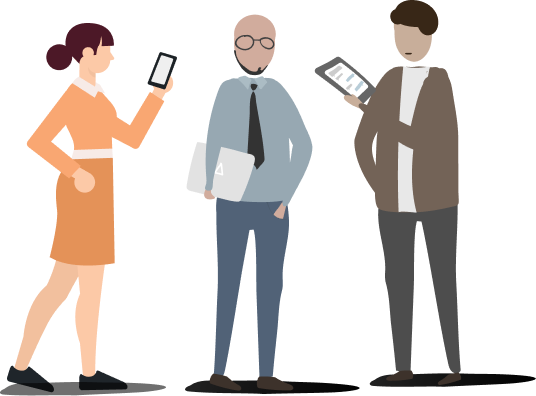
\includegraphics[width=1\textwidth]{images/Users.png}
            \end{figure}
        \end{column}
    \end{columns}
\end{frame}

\begin{frame}{Sharing in collaborative applications}
    \begin{columns}
        \begin{column}{0.6\textwidth}
            \begin{itemize}
                \small
                \item Work object is shared by replication (content and formatting)
                \item Communication is transient (chat)
                \item Tools are individual, but similar across users (UI)
                \item Environment is not shared (browser/extensions)
            \end{itemize}
        \end{column}
        \begin{column}{0.4\textwidth}
            \begin{figure}[h]
                \centering
                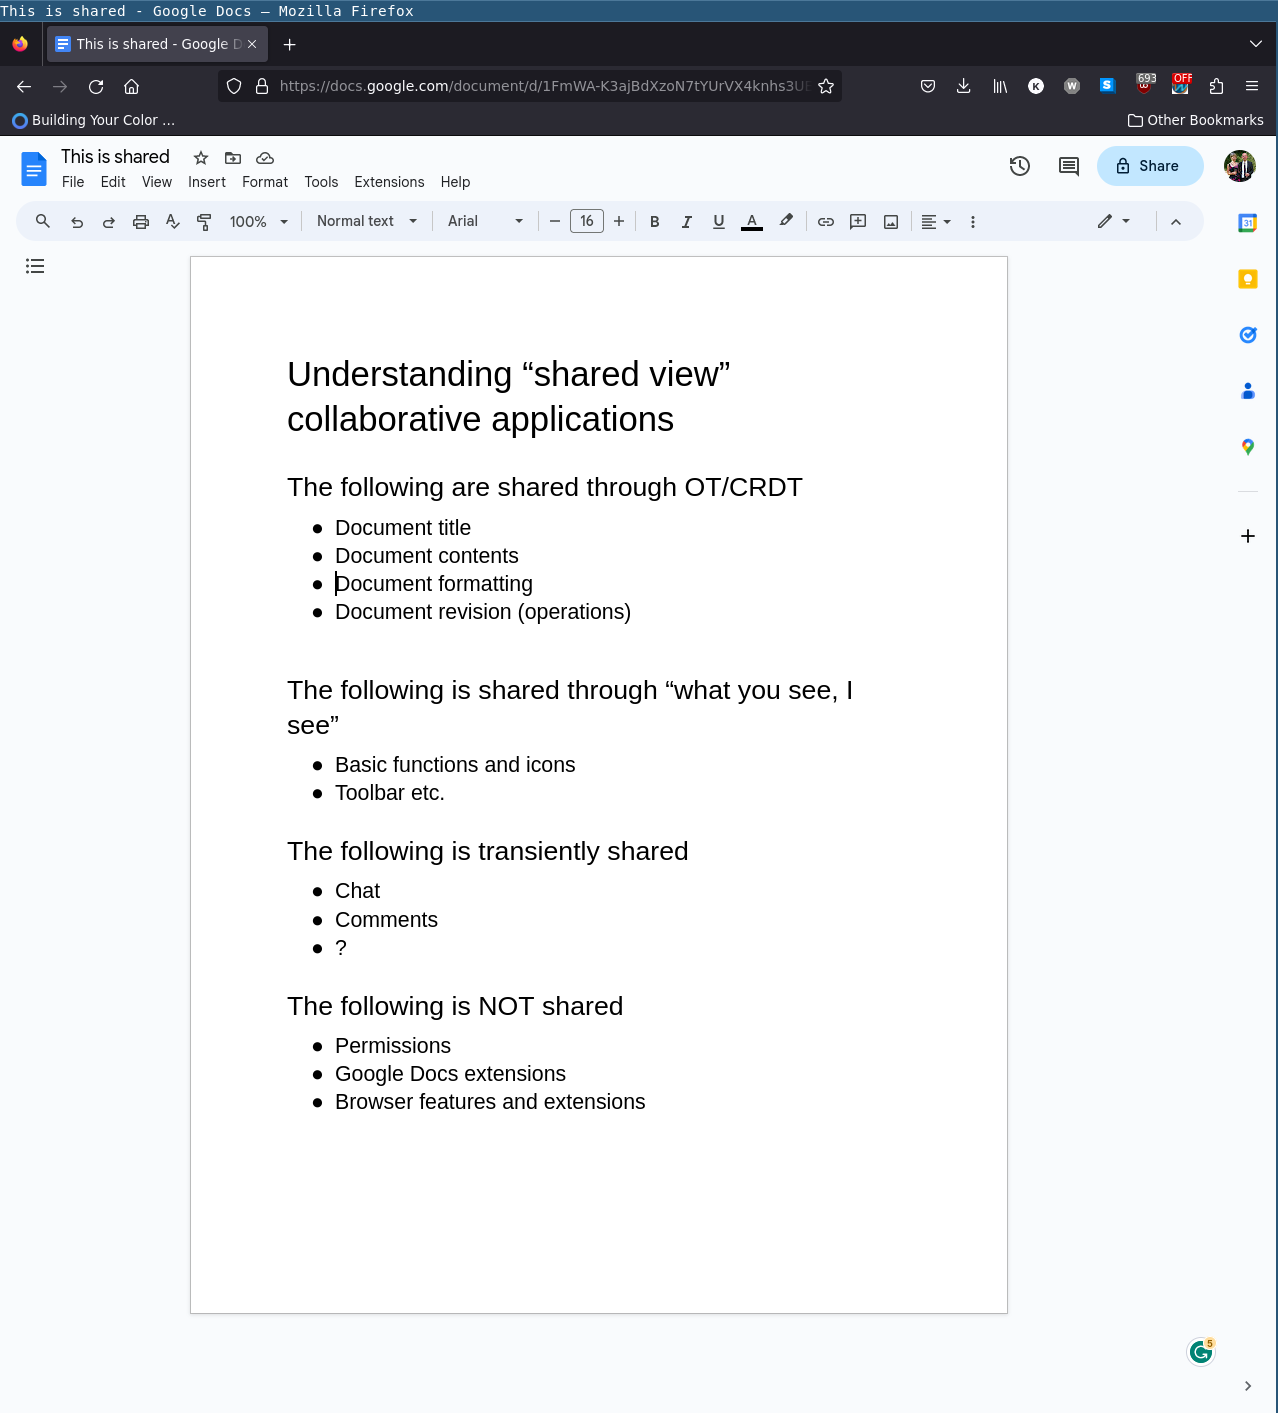
\includegraphics[width=0.8\textwidth]{images/gdocs.png}
                %\caption{Google Documents Sharing Model}
            \end{figure}
        \end{column}
    \end{columns}
\end{frame}

\begin{frame}{Interaction Design features}
    \begin{itemize}
        \item The user can save changes as individual \textbf{views} (sheets) of data
        \item \textbf{The user can share their saved views with other users}
        \item[] $\rightarrow$ The user can add or remove columns from the \textbf{view}
        \item[] $\rightarrow$ Users can filter and order the table content
        \item \textbf{Multiple users must be able to work on the same views simultaneously}
        \item[] $\rightarrow$ The users of the system may be located on multiple locations
    \end{itemize} 
\end{frame}


\begin{frame}{Making `views' first class objects}
    \begin{columns}
        \begin{column}{0.4\textwidth}
            %% sige noget om hvorfor det er en challenge
            \begin{itemize}
                \footnotesize
                \item Data views as the main work object -- it's what is shared when collaborating
                \item Views can be published in formats fitting the consumer needs
                \item A data view encapsulate a data source, users, and the revision history
            \end{itemize}
        \end{column}
        \begin{column}{0.6\textwidth}
            \begin{figure}[h]
                \centering
                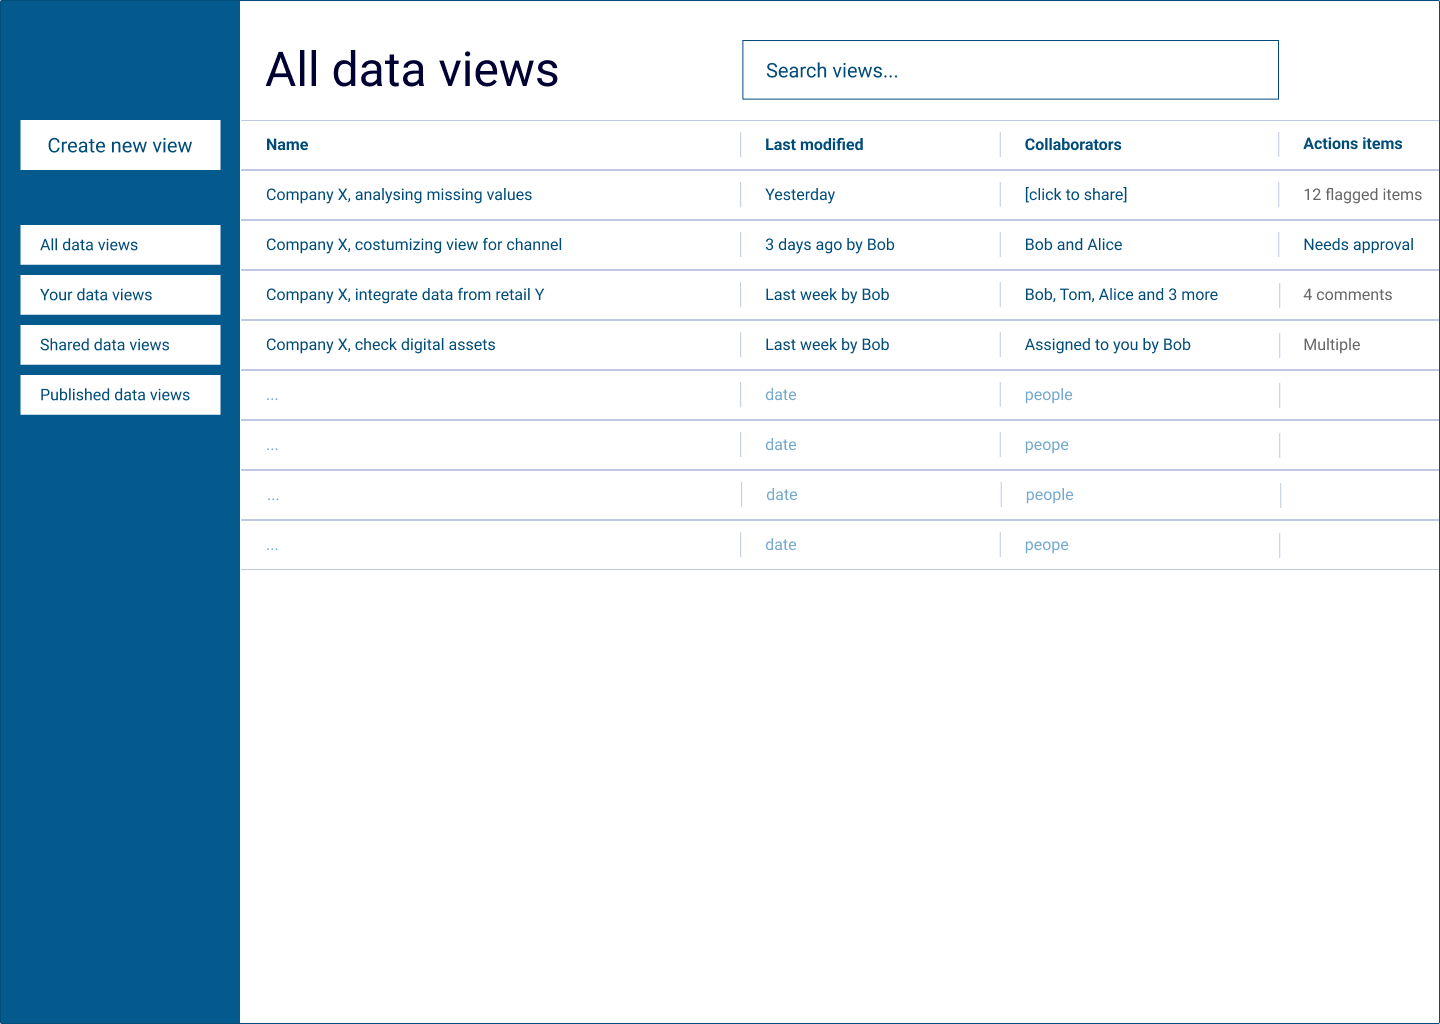
\includegraphics[width=1\textwidth]{images/all-data-view.png}
            \end{figure}
        \end{column}
    \end{columns}
\end{frame}

\begin{frame}{Creating a new data view}
    \begin{columns}
        \begin{column}{0.4\textwidth}
            \begin{enumerate}
                \footnotesize
                \item Select data source(s) (or import)
                \item Preview data 
                \item Add collaborators
                \item Generate view
            \end{enumerate}
        \end{column}
        \begin{column}{0.6\textwidth}
            \begin{figure}[h]
                \vspace{-2em}
                \centering
                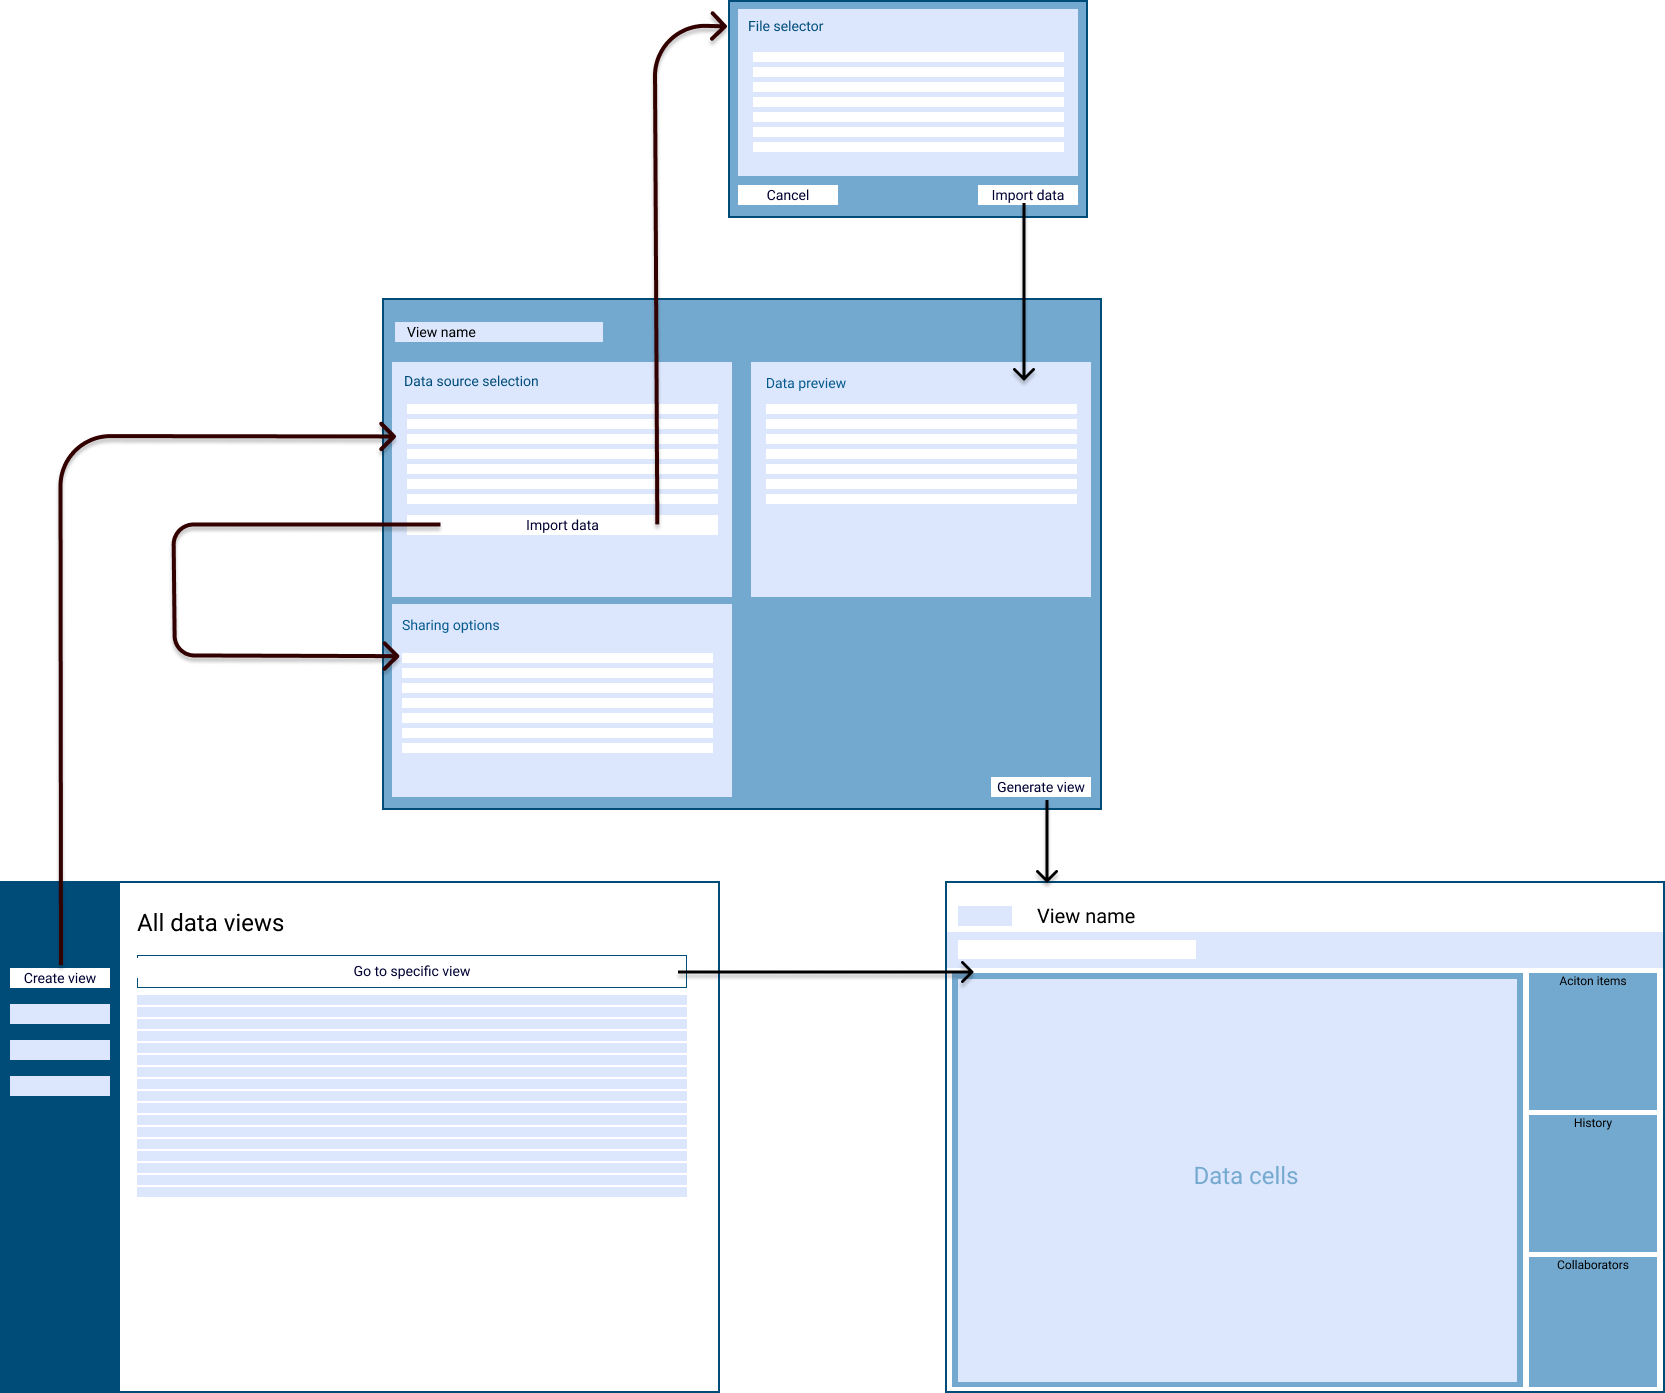
\includegraphics[width=1.1\textwidth]{images/generate-view-flow.png}
            \end{figure}
        \end{column}
    \end{columns}
\end{frame}

%% introduce the view design slide

\begin{frame}{Manipulating shared view}
    \begin{columns}
        \begin{column}{0.6\textwidth}
            \begin{itemize}
                \small
                \item Data operations as the replicated objects:
                \begin{itemize}
                    \footnotesize
                    \item Data manipulation
                    \item View manipulation 
                \end{itemize}
                \item This ensures locatability from history into the changes
                \item \dots and accountability (who did what -- where are we)
                \item Rolling back changes (undo/hide operation)
                \item A set of operations (a macro) can be exported to other data views
                \item (and reviewed before applied to master data)
            \end{itemize}
        \end{column}
        \begin{column}{0.45\textwidth}
            \begin{figure}[h]
                \vspace{-4em}
                \centering
                \includegraphics[width=1\textwidth]{images/sharing-history.png}
            \end{figure}
        \end{column}
    \end{columns}
\end{frame}

\begin{frame}{Collaborating with data views: Assign action item}
    \begin{figure}[h]
        \centering
        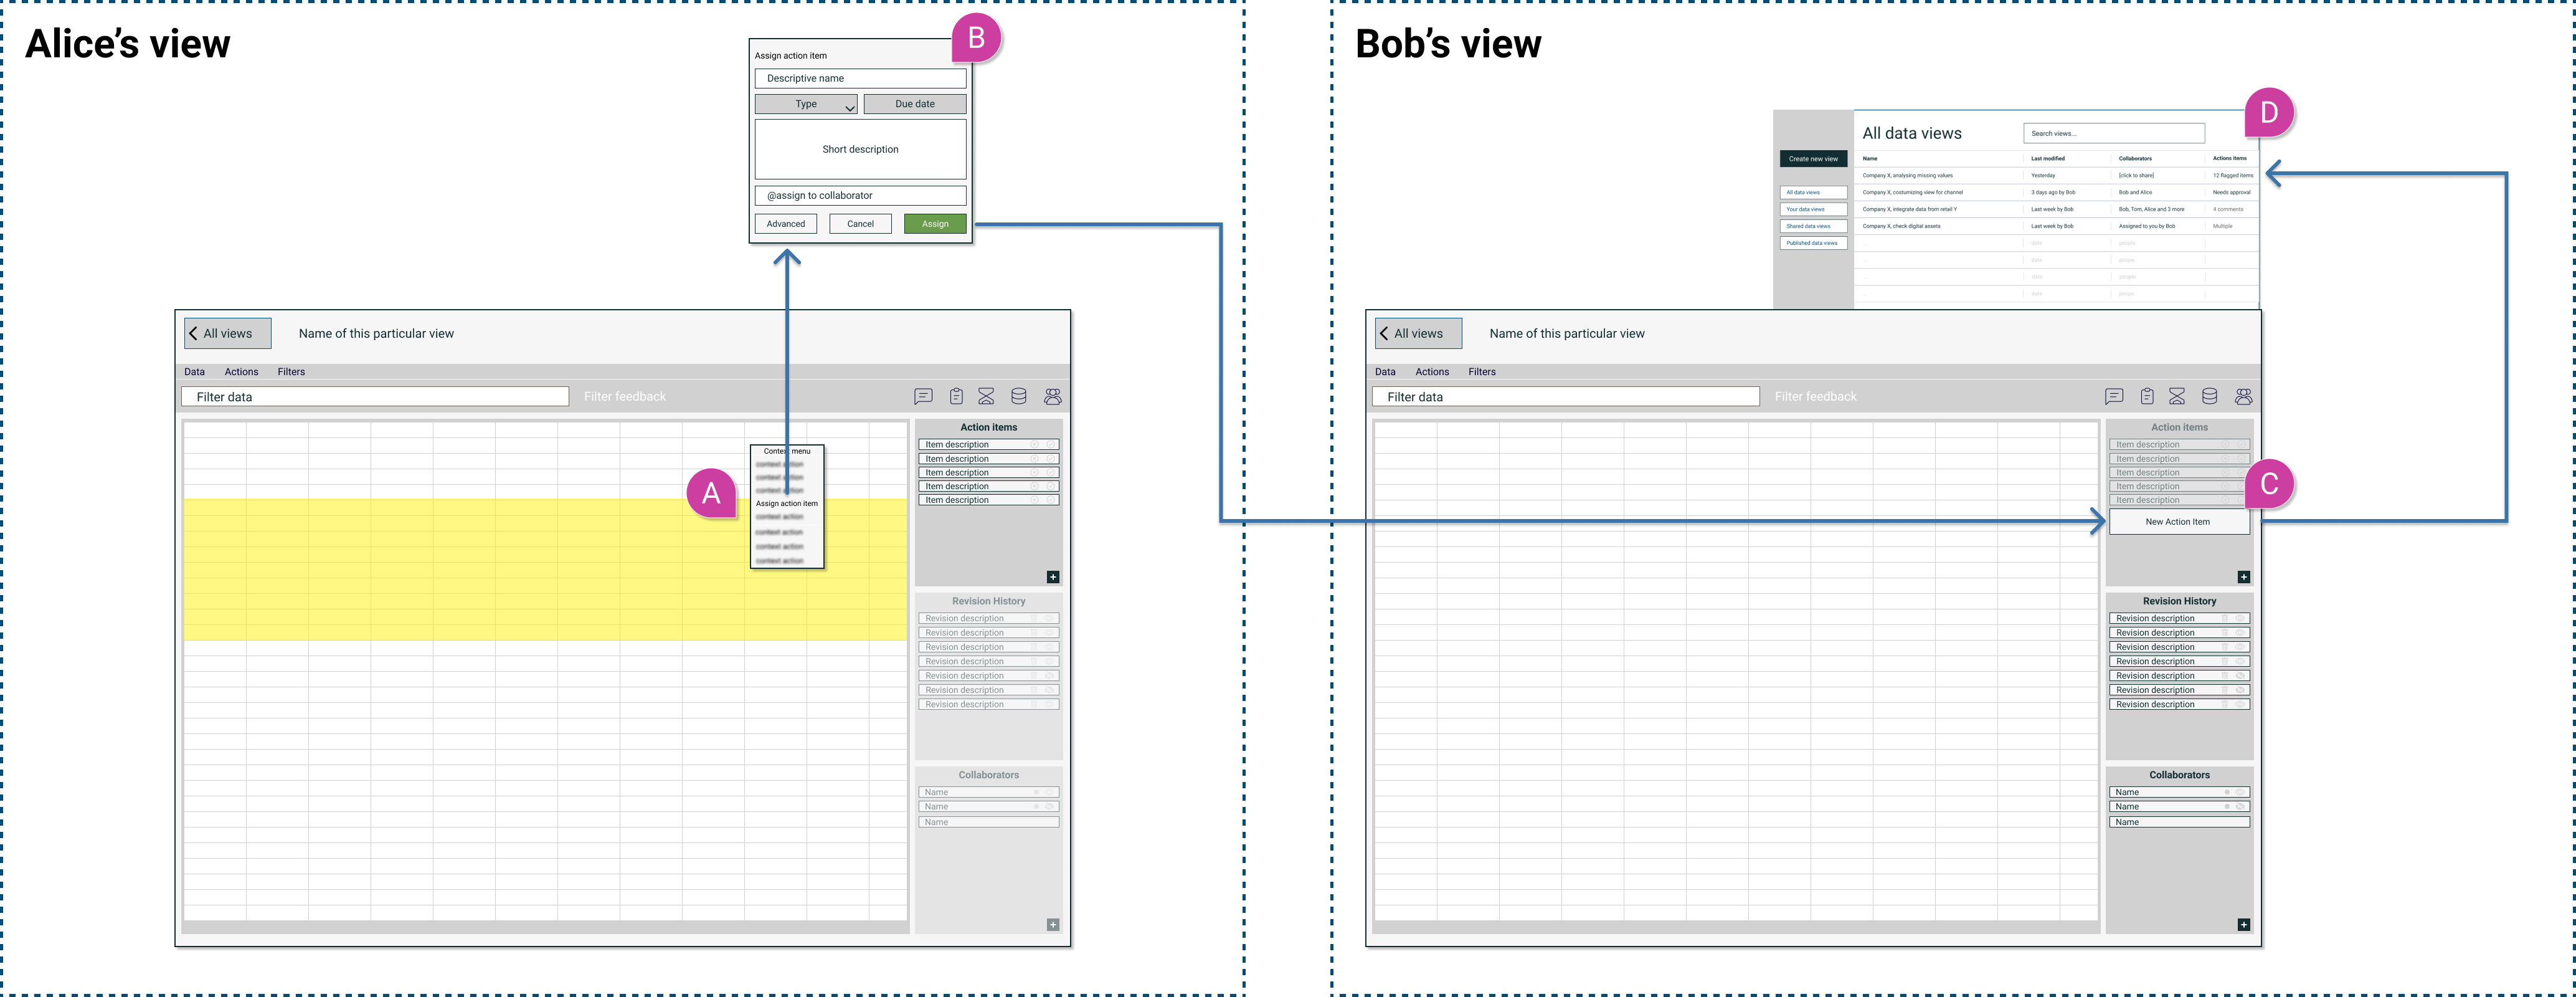
\includegraphics[width=1\textwidth]{images/assign-action-item.png}
    \end{figure}
\end{frame}

\begin{frame}{Key IA/IxD challenges}
    \begin{itemize}
        \small
        \item `Views' might be a difficult concept to grasph for non-data users
        \item Revision history is a difficult concept to get right and powerful for non-programmers
        \item Remote collaboration \textbf{require} additional communication channels
        \item What happens if we add automatisation, quality tests etc. that have delay?
        \item Prototyping (CRDT) collaborative tools pose different requirements than single user applications:
        \begin{itemize}
            \footnotesize
            \item Require more contextual user research and co-design activities
            \item Hard to study from application analytics (but I have done that)
            \item Require some technical infrastructure to prototype collaboration (websockets will get you 80\% there)
        \end{itemize}
    \end{itemize}
\end{frame}
%% I want to explore history
%% I want to explore action items

\end{document}